\section{Results}
\label{sec:results}

All results follow the protocol in Section~\ref{sec:method} and are reported
as mean $\pm$ population standard deviation over three seeds.  The main
comparison in Table~\ref{tab:t1-master-results} uses active budget
$M=2{,}000$ and retrieval budget $b=64$.

\subsection{Main Method Comparison}
\label{subsec:main-comparison}

At the common nominal active budget, Uniform Herding obtains
$44.99\pm1.00\%$ final average accuracy and $13.85\pm0.44\%$ forgetting.
iCaRL obtains $42.36\pm0.87\%$ accuracy and $19.46\pm0.10\%$ forgetting;
the static bank obtains $28.60\pm1.35\%$ and $55.86\pm1.42\%$.
Uniform Herding therefore has higher mean accuracy and lower mean forgetting in
this experiment.  This is an end-to-end comparison of complete protocols:
Uniform Herding retains additional candidates for refresh, while the baselines
retain their nominal active stores, and the methods use different objectives
and readout protocols as specified in the appendix.  Figure~\ref{fig:per-task-accuracy}
shows the corresponding final per-task accuracies.

\begin{table}[t]
  \centering
  \caption{Main comparison on CIFAR-100. All methods use a nominal active
  exemplar budget of 2,000 and retrieval budget 64; Uniform Herding also
  retains candidate storage for refresh.}
  \label{tab:t1-master-results}
  \small
  \resizebox{\linewidth}{!}{%
  \begin{tabular}{lrrr}
    \toprule
    Method & Average accuracy (\%) & Forgetting (\%) & BWT (\%) \\
    \midrule
    iCaRL & $42.36\pm0.87$ & $19.46\pm0.10$ & $-19.46\pm0.10$ \\
    Static bank & $28.60\pm1.35$ & $55.86\pm1.42$ & $-55.86\pm1.42$ \\
    Uniform Herding & $44.99\pm1.00$ & $13.85\pm0.44$ & $-13.54\pm0.39$ \\
    \bottomrule
  \end{tabular}
  }
\end{table}

\begin{figure}[t]
  \centering
  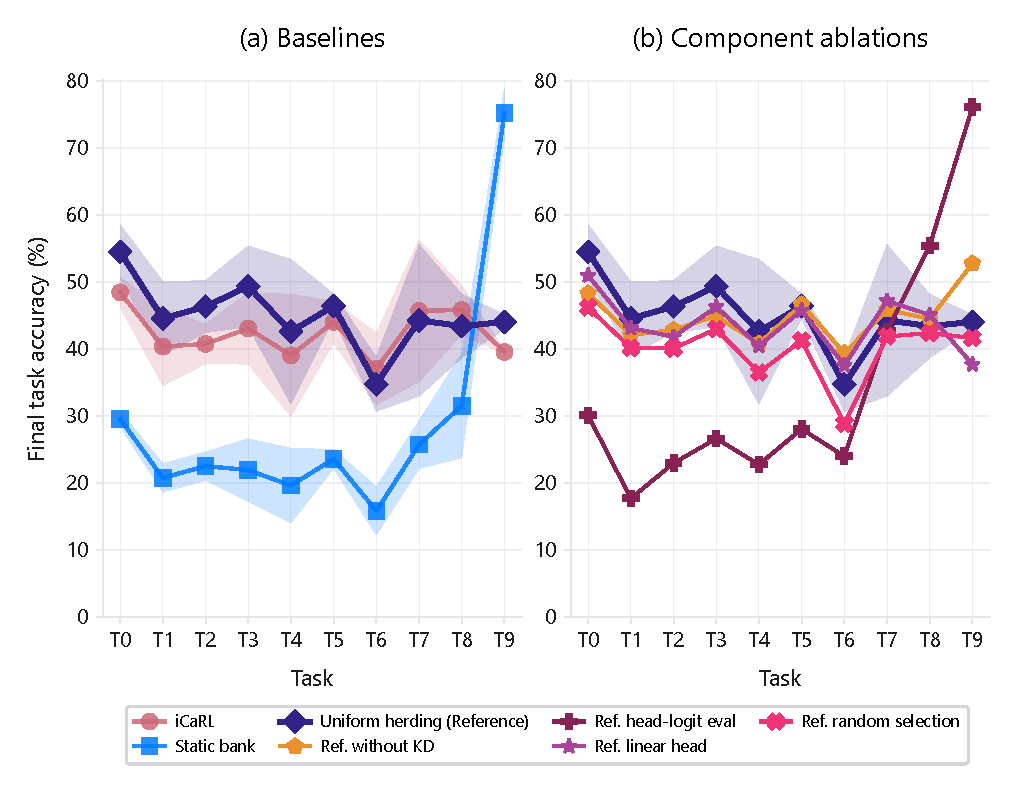
\includegraphics[width=\linewidth]{data/main/figures/fig1_per_task_accuracy.pdf}
  \caption{Final per-task accuracies. Panel (a) compares the baselines with
  Uniform Herding. Panel (b) shows the within-method variants. Shaded bands
  denote population standard deviation over three seeds.}
  \label{fig:per-task-accuracy}
\end{figure}

\subsection{Supporting Analyses of Uniform Herding}
\label{subsec:supporting-analyses}

Table~\ref{tab:t2-component-ablations} reports matched within-method changes
to the prediction rule, selection rule, distillation, and classifier head.
Replacing NME with head-logit evaluation reduces accuracy by $10.38$ pp and
increases forgetting by $32.50$ pp.  Replacing herding with random selection
reduces accuracy by $4.83$ pp and increases forgetting by $4.50$ pp.  Removing
KD changes accuracy by $-0.21$ pp but increases forgetting by $10.93$ pp,
whereas replacing the cosine-margin head with a linear head changes accuracy
by $-1.42$ pp and forgetting by $+0.83$ pp.  These are supporting comparisons
within the stated Uniform Herding protocol, not universal component effects.
Figure~\ref{fig:component-attribution} shows the matched per-seed changes.

\begin{table}[t]
  \centering
  \caption{Matched within-method comparisons for Uniform Herding. Deltas are
  paired by seed against the main configuration.}
  \label{tab:t2-component-ablations}
  \small
  \resizebox{\linewidth}{!}{%
  \begin{tabular}{lrrrr}
    \toprule
    Variant & Average accuracy (\%) & Forgetting (\%) & $\Delta$ accuracy (pp) & $\Delta$ forgetting (pp) \\
    \midrule
    Without KD & $44.79\pm0.31$ & $24.78\pm0.81$ & $-0.21$ & $+10.93$ \\
    Head-logit evaluation & $34.61\pm1.13$ & $46.36\pm1.63$ & $-10.38$ & $+32.50$ \\
    Linear head & $43.57\pm0.47$ & $14.68\pm0.48$ & $-1.42$ & $+0.83$ \\
    Random selection & $40.17\pm0.17$ & $18.35\pm0.61$ & $-4.83$ & $+4.50$ \\
    \bottomrule
  \end{tabular}
  }
\end{table}

\begin{figure}[t]
  \centering
  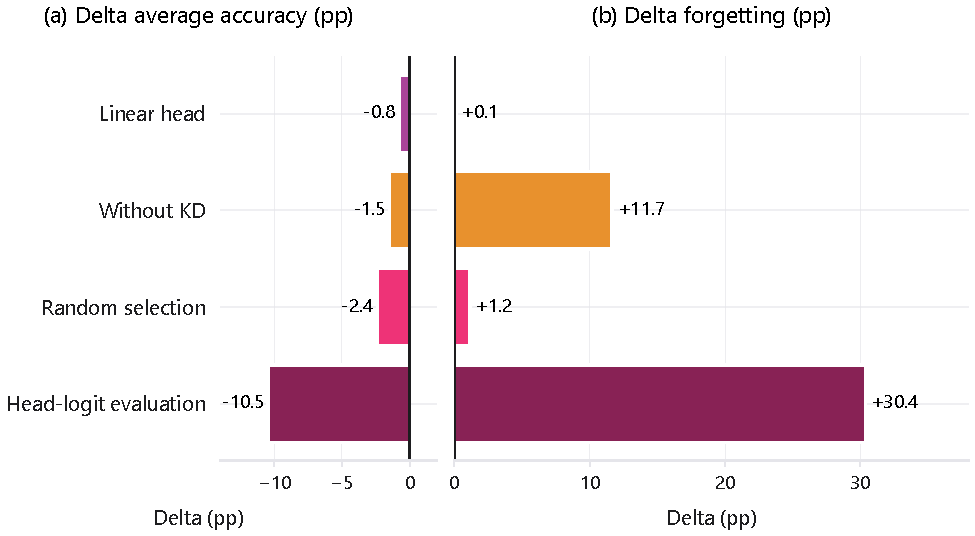
\includegraphics[width=\linewidth]{data/main/figures/fig2_component_attribution.pdf}
  \caption{Matched per-seed changes relative to Uniform Herding. Negative
  accuracy changes and positive forgetting changes are unfavorable.}
  \label{fig:component-attribution}
\end{figure}

\subsection{Active-Budget and Retrieval Sensitivity}
\label{subsec:resource-sensitivity}

Varying the active budget also changes the candidate-pool capacity because
Uniform Herding uses $\rho=3$.  Reducing $M$ from 2,000 to 500 lowers accuracy
by $8.17$ pp and raises forgetting by $5.77$ pp.  Increasing $M$ to 4,000
raises accuracy by $2.66$ pp and lowers forgetting by $1.18$ pp.  These three
points describe a tested-range resource pattern, not a scaling law.

With $M=2{,}000$ fixed, reducing retrieval from 64 to 32 changes accuracy by
$-1.71$ pp and forgetting by $+1.13$ pp.  Increasing retrieval to 128 changes
the corresponding means by $-0.18$ pp and $+0.81$ pp.  The retrieval sweep
therefore shows a smaller mean change over the tested values than the
active-budget sweep (Table~\ref{tab:t3-resource-sensitivity}).
Figure~\ref{fig:resource-sensitivity} visualizes these tested changes.

\begin{table}[t]
  \centering
  \caption{Resource sensitivity relative to Uniform Herding at $M=2{,}000$ and
  retrieval budget 64. Active-budget changes also change the candidate-pool
  capacity through $\rho=3$; deltas are paired by seed.}
  \label{tab:t3-resource-sensitivity}
  \small
  \resizebox{\linewidth}{!}{%
  \begin{tabular}{llrrrr}
    \toprule
    Axis & Value & Average accuracy (\%) & Forgetting (\%) & $\Delta$ accuracy (pp) & $\Delta$ forgetting (pp) \\
    \midrule
    Active budget & 500 & $36.83\pm0.36$ & $19.63\pm1.01$ & $-8.17$ & $+5.77$ \\
    Active budget & 2,000 & $44.99\pm1.00$ & $13.85\pm0.44$ & $0.00$ & $0.00$ \\
    Active budget & 4,000 & $47.66\pm0.72$ & $12.67\pm1.03$ & $+2.66$ & $-1.18$ \\
    Retrieval & 32 & $43.28\pm0.61$ & $14.98\pm0.99$ & $-1.71$ & $+1.13$ \\
    Retrieval & 64 & $44.99\pm1.00$ & $13.85\pm0.44$ & $0.00$ & $0.00$ \\
    Retrieval & 128 & $44.81\pm0.78$ & $14.66\pm0.75$ & $-0.18$ & $+0.81$ \\
    \bottomrule
  \end{tabular}
  }
\end{table}

\begin{figure}[t]
  \centering
  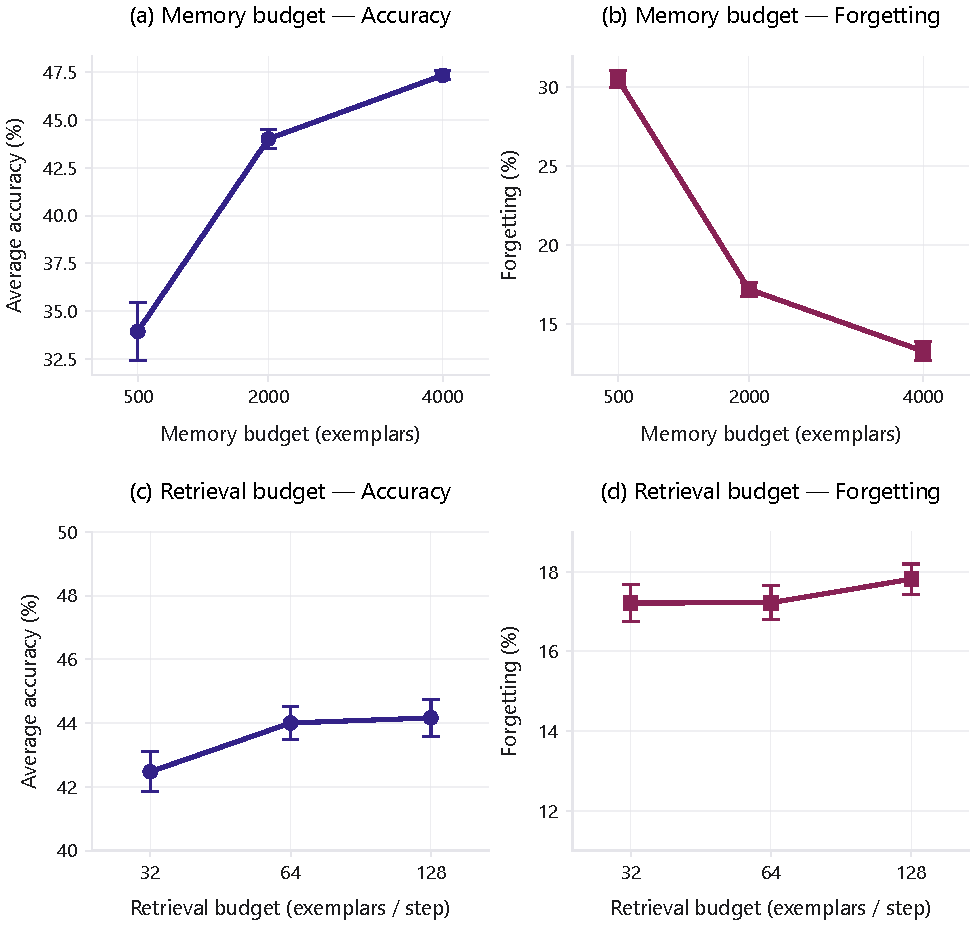
\includegraphics[width=\linewidth]{data/main/figures/fig3_resource_sensitivity.pdf}
  \caption{Sensitivity to active exemplar budget and replay retrieval budget.
  Error bars denote population standard deviation over three seeds.}
  \label{fig:resource-sensitivity}
\end{figure}

\subsection{Accuracy--Forgetting Trade-off}
\label{subsec:accuracy-forgetting-tradeoff}

Figure~\ref{fig:accuracy-forgetting} places the reported configurations in
the accuracy--forgetting plane.  At the common nominal active budget, Uniform
Herding has the highest mean accuracy and lowest mean forgetting among the
three main methods.  The plot is descriptive: its points vary method choices
and resource settings, so they do not define a single causal trade-off curve.

\begin{figure}[t]
  \centering
  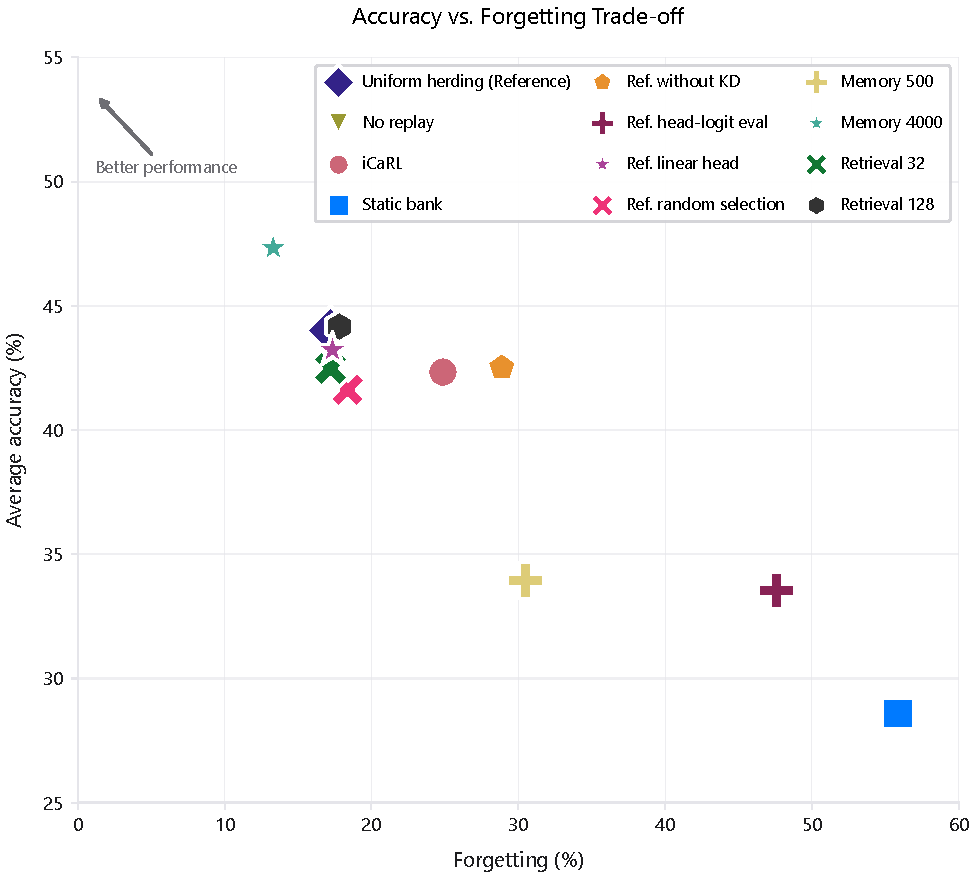
\includegraphics[width=0.92\linewidth]{data/main/figures/fig4_acc_forgetting_scatter.pdf}
  \caption{Average accuracy versus forgetting for baselines, within-method
  variants, and resource configurations. Higher accuracy and lower forgetting
  are preferred.}
  \label{fig:accuracy-forgetting}
\end{figure}

\subsection{Task-Age Failure Modes}
\label{subsec:task-age-failure-modes}

Figure~\ref{fig:forgetting-by-age} shows two contrasting failure modes.  The
static bank incurs approximately $51$--$59$ pp forgetting for tasks 0--8,
whereas head-logit evaluation incurs approximately $25$--$55$ pp.  Uniform
Herding ranges from $7.6$ to $26.8$ pp over these tasks.  In both adverse
configurations, the newest task has higher final accuracy than older tasks,
so aggregate accuracy can conceal recency bias.

The zero forgetting value for task 9 is structural: no later task can reduce
its accuracy under the final-task definition.  It is not evidence that the
last task is retained better than the preceding tasks.

\begin{figure}[t]
  \centering
  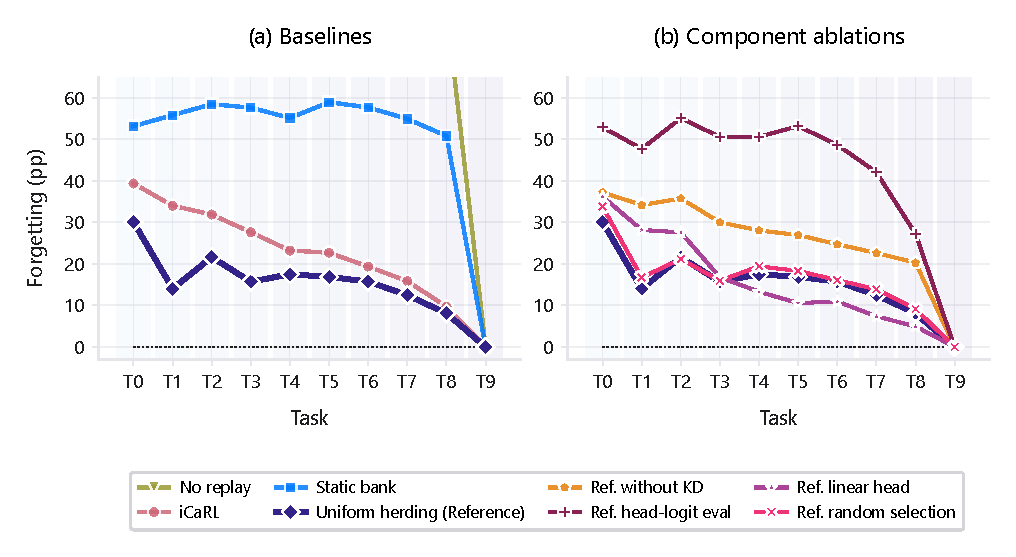
\includegraphics[width=\linewidth]{data/main/figures/fig5_forgetting_by_age.pdf}
  \caption{Forgetting by task index for Uniform Herding and two adverse
  configurations. The final task has zero forgetting by definition because no
  subsequent task is learned.}
  \label{fig:forgetting-by-age}
\end{figure}
